% Some miscellaneous notes:
% I will indicate with my sigil the yellow-folder note pages that I've already
% digitized.

\documentclass[11pt]{article}
\usepackage{reports}

% The following block isn't actually used on the output.
% But it's easier to simply fill it out than to try
% to edit the rather fragile reports.sty file.
\newcommand*{\instr}{Ariel S\'{a}nchez}
\newcommand*{\term}{31.07.2023}
\newcommand*{\coursenum}{Master's Thesis}
\newcommand*{\hwnum}{Redshift Dependence of Neutrino Damping on the Power
Spectrum}

\usepackage{pdfpages}
\usepackage{bm}
\usepackage{listings}
\usepackage{titling}
\usepackage[normalem]{ulem} 

\IfFileExists{biblatex.sty} {
    \usepackage[style=authoryear]{biblatex}
    \addbibresource{master_thesis.bib}
}

% This code formatting sucks but I don't want to output extra spaces.
\newcommand{\cbib}[1]
{\IfFileExists{biblatex.sty}
{\cite{#1}}
{[citation ``#1'' cannot be linked in the current environment]}}

\graphicspath{{./res/}}

\begin{document}

\fontsize{12}{15}

\begin{center}
Lukas Finkbeiner: Master's Thesis
\end{center}

This is a master's thesis. I hope to defend it to your satisfaction.

\tableofcontents

\begin{centering}
\section{Abstract? Summary of Introduction}
\end{centering}

``The goal of this project is to produce an emulator of the linear-theory
power spectrum based on evolution mapping'' (A. G. S\'{a}nchez, private
communication). In particular, this paper seeks to extend the evolution mapping
scheme of \cbib{San21} to massive-neutrino cosmologies by applying a correction
factor to results from emulators built on massless-neutrino simulations. 

\begin{centering}
\section{The Importance of Simulation and Emulation}
\end{centering}

\footnote{
    Some of my ideas for this section strike me as perhaps too introductory.
    The master's thesis is supposed to read like a scientific paper, right?
    But those never start off by talking about LSS nor why it's interesting,
    they just jump right into the novel techniques.
}

We want to study the large-scale structure of the Universe. From our
observations thereof, we want to find the best-fit parameters, such as
the Universe's density in cold dark matter.

If we have a particular cosmology (some specific configuration of these various
parameters) that we would like to explore, it would be helpful to know what
this Universe looks like in the ways that correspond to the capabilities of
our instruments. For example, for any given proposed model, we should like to
know what the power spectrum\footnote{It's a little weird that I'm assuming
familiarity with the power spectrum, given the simplicity used elsewhere.
But I think it's okay.} would look like
in such a Universe so that we
can compare it to the power spectrum that we measure in our own.

To output these kinds of observables based on some proposed model, we task
Boltzmann solvers.

\begin{centering}
\section{Boltzmann Solvers and CAMB}
\end{centering}

This is just a theoretical discussion of these solvers. The hands-on stuff
comes a couple sections later.

``Boltzmann codes account for the baryonic and radiation components of the
energy density as well as for relativistic effects'' (\cbib{Zennaro}).

``In the Newtonian framework often employed in simulations, radiation (photon)
perturbations are neglected, leading to inaccuracies in the power spectrum on
large scales'' (\cbib{Zennaro}). By contrast, Boltzmann solvers do not suffer
from this limitation, right?

Talk about CAMB and CLASS. Are there any important ways in which they
distinguish themselves? Why do we use both of them in modern papers? Anyway,
the reason that we don't use CMBFast (as well as other older codes?) is
because it is no longer maintained.


\begin{centering}
\section{Emulators}
\end{centering}

In order to constrain cosmological parameters based on the application of this
method to \textcolor{red}{LSS data sets}\footnote{
	Vague--you should instead mention the precise names of the data sets,
	and you should even have a dedicated section of the paper wherein you
	summarize the goals, instrumentation, targets, and state-of-the-art
	analyses of these data sets
}, we must call a Boltzmann solver for each point in our parameter space. This
multitude of calls represents an enormous computational, and therefore time,
cost.

Therefore, we would like to build a machine that can predict what the power
spectrum should look like (for any given combination of the input parameters)
based on a relatively small number of input simulations. Emulators have been
recently proposed as such a solution.

\textit{What is an emulator? How do we train it?}
(\cbib{Arico}, \cbib{Mancini}).
At the most basic level, an emulator is an interpolation scheme. ``As the
response of the \uline{non-linear} power spectrum to changes in cosmological
parameters
is smooth, it is possible to build accurate interpolation schemes or emulators,
calibrated on a relatively small number of high-resolution simulations. \sout{
This
technique can also be applied to additional statistics of the density field
such as the halo mass func}'' (\cbib{San21}).
\textcolor{orange}{I underlined ``non-linear'' in the above paragraph because
our focus here, at least at the beginning, is on the \textit{linear} power
spectrum. I imagine the response of the linear power spectrum is also smooth,
but we should make sure of this.}

Most emulators are based on a Gaussian Process (GP). A GP is a Gaussian
distribution over functions\footnote
{A GP is the limit of a one-hidden-layer neural network as the number of
neurons approaches infinity.}, which can be interpreted
as the infinite-dimensional generalization of the multivariate normal
distribution. The inference of continuous values with a GP prior
is known as Gaussian process regression, or Kriging. GP regression is a
powerful non-linear multivariate interpolation tool. The computational
complexity of inference and likelihood evaluation within GP regression is cubic
in the number of points. This makes GP regression an excellent companion to
Latin hypercube sampling (LHS), which demands sparsity.
\textcolor{orange}{Try paraphrasing more deeply, since the above block is still
technically plagiarism even though it wasn't a direct quote. Also, since
``sparsity'' already has a technical meaning,
we should try a different term here.}
``GP-based emulators require fewer training samples than
neural networks but provide smaller speedups. GP's allow natural propagation of
uncertainty in predictions to the final posterior distribution; neural
networks lack this feature'' (\cbib{Mancini}). Actually, that `quote' really
doesn't sound like a direct quote from a paper. \textcolor{orange}{Am I sure I
didn't just write a note in English?}

In GP regression, one makes the assumption that one's data are all
Gaussian-distributed. What are the consequences of this being a bad assumption?

Emulators interpolate across a high-dimensional parameter space. The primary
limitation is that the emulator has to be built with every possible parameter
in mind that an end-user could wish to vary. Yet there is a large number of
different cosmological parameters discussed in the modern literature.
``Currently available emulators only sample a few cosmological parameters,
often with restrictive ranges, and are not applicable to more general parameter
spaces'' (\cbib{San21}). ``Due to the high computational cost of the required
simulations, [...] current emulators leave out parameters such as the curvature
of the Universe or dynamic energy models beyond the standard CPL
parametrization'' (\cbib{San21}).

Now, for a point of suspense: there are so many different cosmological
parameters that we investigate. What is the point of building an emulator if
you just have to train a new one each time you take interest in a new
parameter? This is supposed to be a segue into evolution mapping, a proposed
solution to this problem.

\begin{centering}
\section{Sigma 12 and Evolution Mapping}
\label{sec: sigma_and_evMapping}
\end{centering}

\footnote{
    I have two primary objectives for this section: explain the unit system
    we are using (ditch $h$ factor because it messes up everything--but
    only briefly summarize the main arguments of Sanchez 2020), and briefly
    summarize why we can funnel all of the evolution parameters through
    $\sigma_{12}$ in this way. Unfortunately, this second objective will
    almost certainly require you to bust out a few equations, and even to
    manipulate them a little to tease out relations essential to this paper.
}

Conventional emulator calibration entails the historical units of Mpc / $h$,
but if we use instead units of Mpc, then we can distill all of the evolution
parameters into one parameter, $\sigma_{12}$. Since $h$ is already its own
(shape!) parameter, the conventional $\sigma_8$ parameter is truly a mixture
of two parameters. This presents a host of misleading results  and statistical
ambiguities (\cbib{San20}) which are outside of the scope of this work but
which prompt us to abandon $\sigma_8$.
Similarly, throughout this paper we will refrain from using the conventional
fractional density parameters $\Omega_i$ in favor of the physical density
parameters $\omega_i = \Omega_i h^2$ which similarly eliminate the
dependence on $h$.

(\cbib{San21}) proposes to divide up the full set of cosmological
parameters into two categories: \textit{evolution} parameters $\mathcal{O}_E$
(such as $\omega_b$, $\omega_c$, and $\eta_s$)
affect the amplitude of the power spectrum at a particular redshift, while
\textit{shape} parameters $\mathcal{O}_S$
(such as $\omega_K$, $\omega_\text{DE}$, w(a))
affect the shape of the power
spectrum. \textcolor{orange}{One paper made it sound like shape parameters
affect both shape and amplitude. Was it one of the S\'{a}nchez papers? I think
I misunderstood it, but we have to confirm that we can now understand what was
meant.\footnote{
    I'm certain that I misread this second description, for the following.
    The main \textit{problem} with neutrinos (i.e. why they \textit{don't}
    play nicely with the categories that I am trying to describe here)
    is that they affect \textit{both} shape and evolution! As far as we know,
    the physical density in neutrinos is the \textit{only} parameter that
    is poorly behaved in this way.
}
Why does it help to have these categories in the first place?}\footnote{
    As I understand it, we split the parameters up this way because
    one category of parameters (I think the evolution parameters)
    can be entirely funneled through just one parameter
    (I think it's $\sigma_{12}$, but obviously we should double check that)
}

We take, as the evolution mapping relation for the power spectrum, equation 13
from \cbib{San21}:

\begin{equation}
\label{eq: evMapping_pSpectrum}
    \Delta^2_L (k | z, \Theta_s, \Theta_e)
    =
    \Delta_L^2 (k | \Theta_s, \sigma_{12} \left( z, \Theta_s, \Theta_e \right))
\end{equation}

Why is this scheme important? Evolution mapping\footnote{I think we need to
double check our language here, I think evolution mapping refers to more than
just the categorization scheme} greatly simplifies the emulator
implementation. Because we can
funnel all of the evolution parameters through $\sigma_{12}$, we've effectively
collapsed an entire category of parameters to just one parameter. Fewer
parameters means that we get a faster emulator.

``At the linear level, all models characterized by identical shape parameters
and the same values of the parameter combinations $b \sigma_{12}(z)$ and
$f \sigma_{12}(z)$ will be identical'' (\cbib{San21}).

Anticipating a counterargument: ``For a general cosmology, $h$ is a combination
of shape and evolution parameters. However, for a $\Lambda$CDM Universe, fixing
the values of the shape parameters $\omega_b$ and $\omega_c$ and varying $h$
corresponds to assuming different values of the purely evolutionary parameter
$\omega_\text{DE}$'' (\cbib{San21}).

From my original assignment email:
``If the dependence of the transfer function, $T(k)$, on the relevant physical
density parameters is emulated, it is possible to obtain a prediction for the
full power spectrum in Mpc units for any choice of evolution parameters and
redshift. The full shape of $P_L(k|z)$ can be obtained from the output of the
emulator of $T(k)$ and $n_s$ (and any additional shape parameter controlling
the scale dependence of the primordial power spectrum). The correct amplitude
of $P_L(k|z)$ can be obtained by computing the value of $\sigma_{12}(z)$ in
terms of the desired normalization at $z=0$ and the growth factor $D(z)$ for
the cosmology being considered. Such a recipe would be valid for a wide range
of evolution cosmological parameters, including non-standard models, as long as
the corresponding linear growth factor is scale-independent. The smaller number
of parameters required to emulate $T(k)$ would increase the overall accuracy of
the predictions while avoiding the need to sample the redshift evolution of
$P_L(k|z) P_L(k|z)$ explicitly would greatly simplify the calibration
procedure'' (A. G. S\'{a}nchez, private communication).

\textcolor{orange}{I believe that $P_L(k|z) P_L(k|z)$ is a typo in the above
paragraph, but I don't know how else to transcribe Ariel's email. Maybe he
made a mistake?}

``The time evolution of $\Delta_L^2(k)$ in models with identical shape
parameters
but different evolution parameters can be mapped from one to the other by
relabelling the redshifts that correspond to the same clustering amplitude
(i.e. $\sigma_{12}(z)$)''.
(\cbib{San21}).

Now, for the hiccup: this scheme is broken by one parameter, the Universe's
density in neutrinos. (In the next section: why this is so and what we can do
about it.)


\begin{centering}
\section{Neutrinos and Their Cosmological Impact}
\end{centering}

\footnote{
    Here I am violating my traditional rule of ordering sections by
    increasing complexity, because I consider the $\sigma_{12}$ argument
    decidedly more esoteric than a summary of the relevant points of neutrino
    physics. I think we should stick with this structure though, in the
    interest of narrative. Specifically, neutrinos represent a wrench in the
    plan. For that development to make sense, we first need to have established
    what
    the ``plan'' is: evolution mapping.
}

(\cbib{Kiakotou}): ``Neutrinos with masses on the eV scale or below will be a
hot component of the dark matter and will free-stream out of overdensities and
thus wipe out small-scale structures.''

``In general, a larger density of relativistic species leads to a smaller
growth of matter fluctuations'' (\cbib{Zennaro}).

``Thermal velocities dominate neutrino dynamics during the first time-steps
(after $z=99$), having a dispersion roughly five orders of magnitude larger
than the dispersion of peculiar neutrino velocities.''

The evolution of neutrino density, like that of photon density, depends on the
momentum distribution.

\begin{equation}
    p_{\nu, i}(z)
    =
    \frac{(k_B T_{\nu, 0})^4}{\pi^2}
    \,
    (1 + z)^4
    \,
    \mathcal{F} \left[ \frac{m_{\nu, i}}{k_B T_{\nu, 0} (1 + z)} \right]
\end{equation}

where $i$ indexes the neutrino species and

\begin{equation}
    \mathcal{F}(y) \equiv \int_0^\infty \frac{x^2 \sqrt{x^2 + y^2}}{1 + e^x}
\end{equation}

 (\cbib{Zennaro})

``The two-fluid approximation consists in assuming that neutrino perturbations
are well described by two variables: density and velocity divergence''
(\cbib{Zennaro}).

Remember what the point of this section is: why is $\omega_\nu$ bad for the
evolution mapping scheme? Because neutrinos exhibit redshift-dependent
damping of the power-spectrum, and therefore affect both the shape and the
amplitude of the power spectrum. Whenever massive neutrinos are present,
the growth factor becomes scale-dependent, which disrupts the
evolution-mapping scheme.

Why? I \textcolor{orange}{think} that it's because all neutrinos start off as
relativistic particles in the early Universe, acting as a type of radiation.
But as the Universe continues to expand and cool, the neutrinos behave
increasingly like dark matter.
In this way, the physical density in neutrinos impacts both the shape and the
evolution. What I don't understand is why we say that this is so when we
only ever consider the shape of the power spectrum at one redshift. By
``shape'' I was assuming that S\'{a}nchez meant the shape of $P(k)$ versus
$k$ but if $\omega_\nu$ is really a problem, then shape should also refer
to $P(k)$ through all values $z$? I don't quite understand this, but
\textcolor{green}{maybe we can ask Ariel}.

``The scale where the suppression of power (from neutrino free-streaming) sets
in is controlled by the comoving Hubble radius at the time when the neutrinos
became non-relativistic, corresponding to a comoving wave number
$k_{fs} = 0.10 \Omega_m h \sqrt{f_\nu}$.

``The popular heuristic formula for the linear theory suppression of the matter
fluctuations by free-streaming $\nu$, $\Delta P(k) / P(k) \approx -8 f_\nu$, is
valid only on very small scales $k > 0.8 h$ / Mpc, However, it is not of
practical use as this is in the strongly nonlinear regime of matter
clustering'' (\cbib{Kiakotou}).

One proposed solution is to treat the neutrinos as a small correction factor
to the results from an anologous cosmology with the same $\omega_m$ but with
$\omega_\nu = 0$. This of course limits the applicability of our emulator to
cosmologies with very small $\omega_\nu$, but this constraint agrees with
current observations (\textcolor{orange}{which?}).


\begin{centering}
\section{CAMB, Initial Setup}
\end{centering}
\footnote{
    At this point, we've built suspense in the reader: we have a goal and
    we have an idea about how to get to that goal. Therefore, now is the
    appropriate time to divert into laying the technical groundwork which
    will allow us to explore our idea through concrete implementations and
    to test our idea with plots and numbers.
}

CAMB is a Fortran code with a Python wrapper\footnote{
\url{https://github.com/cmbant/CAMB}
}which we will be using for the
entirety of this project.

To introduce the reader to the scope of CAMB, we will now introduce
some basic simulated power spectra along with a summary of the dynamic
parameters which will be of greatest interest to us.

Neutrino mass hierarchy: the options are degenerate, normal, and inverted.
The CAMB documentation annotates this parameter as ``(1 or 2 eigenstate
approximation),'' but this is somewhat unclear. Is the degenerate
hierarchy the single mass eigenstate approximation? Do both normal
and inverted hierarchies involve two eigenstates?

I guess we could already start putting a couple of plots here from my existing
notebooks. I mean, I'm sure none of these plots will survive to the final
version, but they might help to guide my discussion for a little while.

IN THIS NEXT SECTION WE WILL BE DISCUSSING SOME OF THE VARIOUS CAMB SETTINGS
AND THE STANDARD VALUES THAT WE USE, INCLUDING BRIEF ILLUSTRATIONS OF THE
SIGNIFICANCE OF EACH SETTING BY WAY OF EXAMPLE ERROR PLOTS WHEN NONSTANDARD
VALUES ARE USED.

In figure \ref{fig: spectrum_type}, we can see that requesting of the wrong
power spectrum type can in some low-$\omega_\nu$ cases yields errors so low
that we might accidentally overlook them. This error pattern is easily
recognizable and is a consequence of the definition of the power spectrum: the
Fourier transform  of the two-point correlation function.
\textcolor{red}{If we
have more matter overall, we expect larger correlations.
WE DON'T HAVE MORE MATTER! That's the whole point of the MEMNeC. The amount of
matter is the same, but cold dark matter clumps more on smaller scales than
neutrinos do. Wait, sorry, I'm confusing myself. We're talking about just one
model THEN we look at two different spectra types. Sorry.
}
Furthermore, the impact of decreasing redshift is only to shift the inflection
point towards larger scales.

\begin{figure}
    \centering
    \begin{minipage}[t]{.49\textwidth}
        \raggedleft
        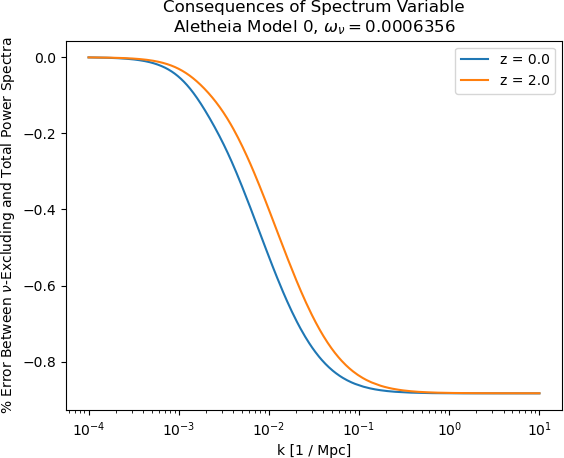
\includegraphics[width=0.99\textwidth]{line_by_line/spectrum_variable/low_omnuh2}
    \end{minipage}
    \begin{minipage}[t]{.49\textwidth}
        \raggedright
        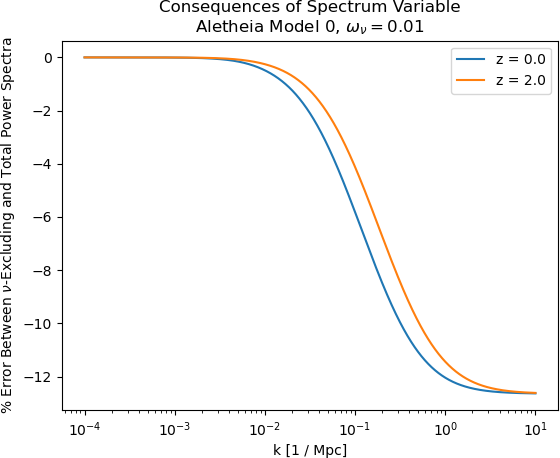
\includegraphics[width=0.99\textwidth]{line_by_line/spectrum_variable/high_omnuh2}
    \end{minipage}
    \caption{Left: small Right: big}
    \label{fig: spectrum_type}
\end{figure}

\begin{centering}
\section{MCMC}
\end{centering}

\textit{What is the MCMC?} Monte Carlo Markov Chain is a way of exploring this
parameter space in the interests of finding the best fit parameters, right?
It is esesntially a random walk in parameter space (\cbib{Verde}).
Should this definition come
when we're trying to use our emulator to make conclusions about our data?
So, the paper that Ariel gave me on this talks about fitting to the WMAP
CMB data with MCMC running on some likelihood function. Is there ever a point
at which I'm actually making a conclusion about the world, or am I just
constructing a tool here by studying the redshift dependence of neutrinos?

``A properly derived and implemented MCMC draws from the joint posterior
density $\mathcal{P}(\alpha | x)$ once it has converged to the stationary
distribution'' (\cbib{Verde}).

``The MCMC method scales approximately linearly with the number of parameters''
(\cbib{Verde}).

There are always areas of the target distribution that have not been covered by
a finite Markov chain. If the chain does not move rapidly throughout the
support of the target distribution because of poor \textit{mixing}, a full
exploration of the likelihood surface might take a prohibitive amount of time.
Degeneracies and poor parameter choices slow the rate of the convergence and
mixing, because the chain spends time exploring degeneracy directions
(\cbib{Verde}). Therefore, our evolution mapping approach comes in handy here
as well, because we eliminate the degeneracies of evolution parameters with
each other!

One of the advantages associated with the MCMC technique is the increased
robustness that follows from the averaging of a large number of points. By
contrast, ``grid-based likelihood calculations and methods that numerically
calculate the Fisher matrix'' are typically more sensitive (\cbib{Verde}).

\textcolor{orange}{Do you want to discuss the Metropolis-Hastings algorithm at
all? Maybe just a brief outline as a motivation?}


\begin{centering}
\section{COMET}
\end{centering}

With this section, we would like to briefly introduce the particular emulation
suite with
which this paper will deal. COMET implements evolution mapping as introduced
by \cbib{San20} and \cbib{San21}, introduced in section
\ref{sec: sigma_and_evMapping}.

\begin{centering}
\section{Analysis}
\end{centering}

``Applying the emulator to a complete inference analysis from a simulated
survey is a necessary step to ensure that the tool can be safely applied in
practical analyses. Checking residuals in the testing set between predicted and
real spectra is not a sufficient accuracy test. While an emulator may be
performing with e.g. sub-percent accuracy at the level of residuals, this may
still not be enough to retrieve unbiased cosmological contours''
(\cbib{Mancini}).

\begin{centering}
\section{Conclusion and Thoughts for the Future}
\end{centering}

``A relation similar to eq. 13 [here reproduced as equation
\ref{eq: evMapping_pSpectrum}] must be valid
for higher-order N-point statistics, geometrical and topological descriptors
such as Minkowski functionals, or the full probability distribution function of
the density field'' (\cbib{San21}). So, the correction factors that we have
introduced in this paper shall surely maintain relevance as we expand our
emulators to handle other cosmological statistics.

\begin{centering}
\section{Dumpster}
\end{centering}

\footnote{
    The following is a giant dumpster (\textit{NOT} a graveyard) for notes
    that I took on paper, as well as possible directions in which to take the
    report. I hope to eventually organize these into a coherent story.

    What with the introduction of so many
    sections, this dumpster acts as a miscellaneous
    temporary storage location. If the note appears here, that implies that I
    didn't know where else to put it. So, it may be that many of these notes
    are ultimately deemed insufficiently relevant to the report...
}

``Perturbation theory breaks down at small scales and low $z$, at least for
nonlinear evolution of structures'' (\cbib{Zennaro}).

$f(k) \equiv \frac{d \ln D(k, a)}{d \ln a}$ where $\delta(a) = \delta_i D(a)$.

GR predicts that $f(k) \approx \Omega_m^{0.55}$ (\cbib{Zennaro}).

``The deviations between the non-linear power spectra of models with identical
$\Delta_L^2 (k)$ caused by their different structure formation histories are
described in terms of the suppression factor $g(a) = D(a) / a$''
(\cbib{San21}).

``Present-day measurements of the CMB alone can accurately constrain the values
of most of the shape parameters. However, they only provide weak constraints on
the evolution parameters for general cosmologies. The inverse is true for LSS
measurements.

``A good approximation even for non-standard cosmologies: perturbation theory
kernels are independent of cosmology'' (\cbib{San21}).

``The fundamental assumption of single-stream flow of common perturbation
theory approaches eventually breaks down due to shell crossings on small
scales'' (\cbib{San21}). Actually I have no idea what this quote means, but
since \cbib{San21} is so important to this paper, I feel like \textcolor
{orange}{I ought to}.

``Several studies have shown that $f(\sigma)$ cannot be described by a
universal function at high accuracy as its amplitude and shape are cosmology
and redshift dependent'' (\cbib{San21}).

``When using the MCMC technique, the values of all evolution parameters are
treated as slow quantities that require a new call to a Boltzmann solver every
time their values are changed'' (\cbib{San21}).

``As a rule of thumb, the present-epoch matter power spectrum is considered to
be in the linear regime for comoving wave numbers $k < $ 0.10--0.15 $h$
Mpc$^{-1}$'' (\cbib{Kiakotou}).

``Nonlinearities introduce a coupling between large and small scales''
(Zennaro et al, 2017).

``The leading-order low-$z$ astrophysical effect [on the microwave sky] is
expected to be gravitational lensing of the CMB by foreground structures; this
generates a $<1$\% covariance in the $\pi$ angular power spectrum on WMAP
angular scales'' (\cbib{Verde}).

``The power spectrum covariance encodes the uncertainties in the power spectrum
due to cosmic variance, detector noise, point sources, the sky cut, and
systematic errors'' (\cbib{Verde}).

\begin{centering}
\section{Meta / Lessons Learned}
\end{centering}

\footnote{Normally, meta comments go in the pretty notes file. This is an
exceptional case for any lessons that specifically guide the writing of this
this paper, and in the final report I hope that I could talk about the
intuition behind these kinds of lessons. For example, I plan to eventually
migrate some of the cases from the ``Lessons in Appraisal'' section of the
pretty notes to this area.
}

\IfFileExists{biblatex.sty} {
    \printbibliography
}

\end{document}
